\chapter{Consuntivo}\label{chap:consuntivo}
In questa sezione del documento sono riportati i consuntivi orari ed economici di ogni sprint, frutto dell'effettivo grado di avanzamento di questo progetto.\\
A facilitare la lettura dei dati, le tabelle dei consuntivi orari ed economici sono accompagnate da grafici riportanti la distribuzione dei ruoli per membro in uno sprint e il budget rimanente in relazione al costo effettivo.\\ \\
Nel consuntivo orario, così come per i preventivi, i ruoli vengono riportati con le seguenti abbreviazioni:
\begin{itemize}
    \item R.: responsabile;
    \item Am.: amministratore;
    \item Pj.: progettista;
    \item An.: analista;
    \item Pg.: progettista;
    \item V.: verificatore.
\end{itemize}
Ogni consuntivo di periodo è accompagnato da un'analisi retrospettiva elaborata durante una riunione interna di fine sprint, le cui considerazioni saranno riflesse in aggiornamenti della pianificazione, dei tempi e dei costi preventivati qualora necessario.
\newpage


\section{Requirements and Technology Baseline}

\subsection{Primo sprint: 2023/11/06 - 2023/11/19}

\subsubsection{Consuntivo orario}
{
\setlength{\tabcolsep}{10pt}
\renewcommand{\arraystretch}{1.5}
\rowcolors{2}{oddrow}{evenrow}
\begin{table}[h!]
    \centering
    \begin{tabularx}{\textwidth}{| l | c | c | c | c | c | c | X |}
        \hline
        \rowcolor{headerrow} \textbf{\textcolor{white}{Membro}} & \textbf{\textcolor{white}{R.}} & \textbf{\textcolor{white}{Am.}} & \textbf{\textcolor{white}{Pj.}} & \textbf{\textcolor{white}{An.}} & \textbf{\textcolor{white}{Pg.}} & \textbf{\textcolor{white}{V.}} & \textbf{\textcolor{white}{Totale}} \\
        \hline
        Anna Nordio & - & 2 & - & 2 & - & 5 & \textbf{9} \\
        \hline
        Giovanni Menon & 7 & - & - & 1 & - & - & \textbf{8} \\
        \hline
        Leonardo Lago & - & 2 & - & 6 & - & 1 & \textbf{9} \\
        \hline
        Marco Dolzan & - & 1 & - & 6 & - & 2 & \textbf{9} \\
        \hline
        Francesco Ferraioli & - & 9 & - & - & - & 1 & \textbf{10} \\
        \hline  
        Francesco Giacomuzzo & - & 1 & - & 2 & - & 4 & \textbf{7} \\
        \hline
        Andrea Cecchin & - & 1 & - & 8 & - & 1 & \textbf{10} \\
        \hline
    \cellcolor{headerrow} \textbf{\textcolor{white}{Totale}} & \textbf{7} & \textbf{16} & - & \textbf{25} & - & \textbf{14} & \textbf{62} \\
        \hline
    \end{tabularx} 
    \caption{Consuntivo orario primo sprint}
    \label{tab:consuntivoorarioprimosprint}
\end{table}
}
{
\begin{figure}[h!]
    \centering
    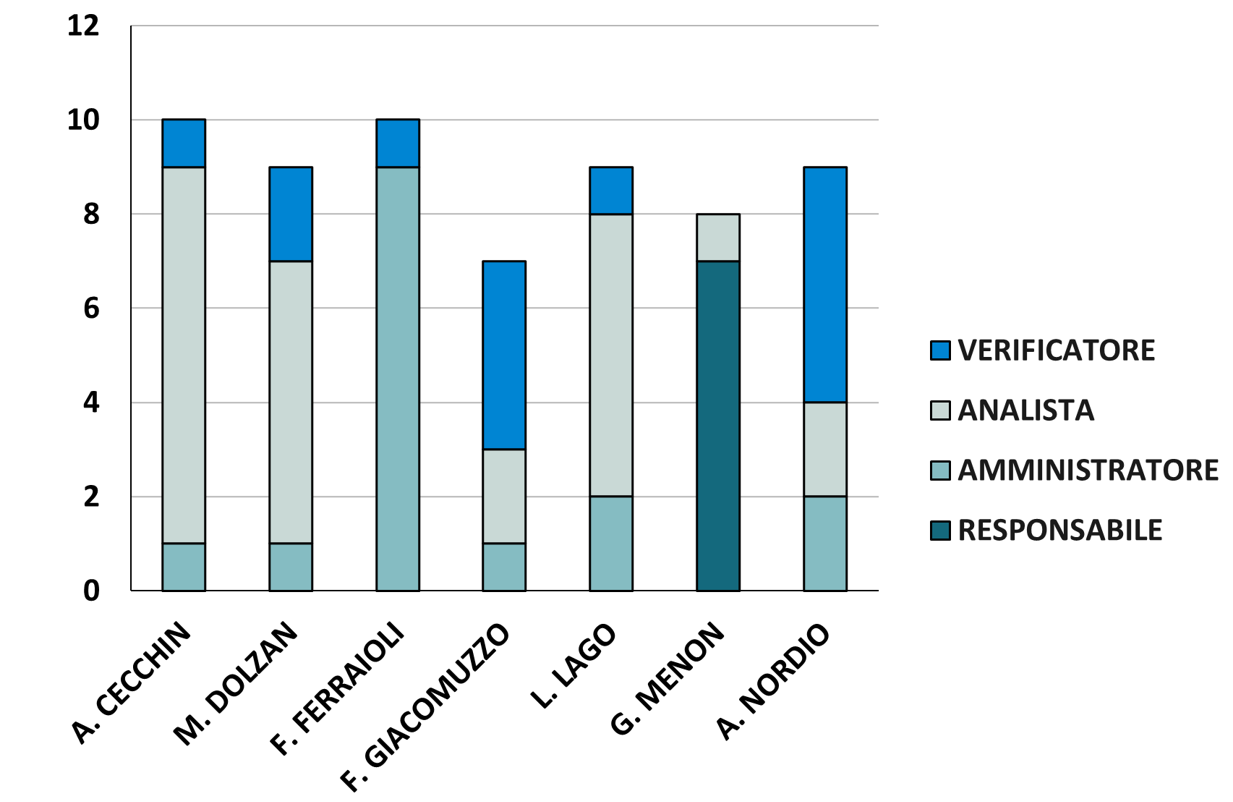
\includegraphics[width=0.8\textwidth]{cons1ruoli.png}
    \caption{Ruoli effettivi primo sprint}
    \label{fig:consuntivootarioprimosprint}
\end{figure}
}
\newpage

\subsubsection{Consuntivo economico}
{
\setlength{\tabcolsep}{10pt}
\renewcommand{\arraystretch}{1.5}
\rowcolors{2}{oddrow}{evenrow}
\begin{table}[h]
    \centering
    \begin{tabularx}{\textwidth}{| l | l | l | X |}
        \hline
        \rowcolor{headerrow} \textbf{\textcolor{white}{Ruolo}} & \textbf{\textcolor{white}{Costo orario}} & \textbf{\textcolor{white}{Ore impiegate}} & \textbf{\textcolor{white}{Costo €}} \\
        \hline
        Responsabile & 30 & 7 & 210\\
        \hline
        Amministratore & 20 & 16 & 320\\
        \hline
        Progettista& 25 & 0  & 0\\
        \hline
        Analista & 25 & 25  & 625\\
        \hline
        Programmatore & 15 & 0  & 0\\
        \hline
        Verificatore & 15 & 14  & 210\\
        \hline
        \cellcolor{headerrow} \textbf{\textcolor{white}{Totale}} &  &  & \textbf{1365}\\
        \hline
        \cellcolor{headerrow} \textbf{\textcolor{white}{Rimanente}} &  &  & \textbf{11620}\\
        \hline
    \end{tabularx}
    \caption{Consuntivo economico primo sprint}
    \label{tab:consuntivocostiprimosprint}
\end{table}
}
{
\begin{figure}[h!]
    \centering
    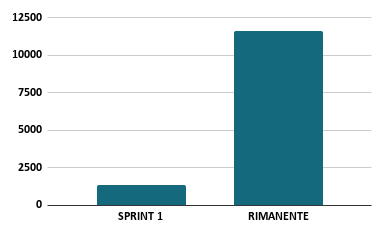
\includegraphics[width=0.8\textwidth]{cons1costo.png}
    \caption{Costo primo sprint e rimanente}
    \label{fig:consuntivocostoprimosprint}
\end{figure}
}
\newpage

\subsubsection{Analisi retrospettiva}
Analizzando le ore impiegate nel primo sprint, in relazione allo stato di avanzamento del progetto, il precedente periodo risulta essere positivo nel suo complesso. Da un'analisi collettiva è emersa una difficoltà da parte dei verificatori di svolgere il loro lavoro minimizzando quanto più il discostamento tra ore produttive e di orologio: questo a causa di una non sempre ottimale comunicazione interna al gruppo. Non è tuttavia ritenuta una questione di cui allarmarsi, in quanto l'elevato numero di ore impiegate nel ruolo di amministratore hanno portato alla realizzazione di \ccgloss{automazioni} a sostegno del lavoro di ogni membro. Con la possibilità di utilizzare l'ambiente di project management di \ccgloss{Jira} al massimo del suo potenziale nel prossimo sprint, si è sicuri di ottimizzare la distribuzione di task e diminuire il rapporto tra ore produttive e ore di orologio già citato.\\
Il massiccio impiego di analisti ha portato il documento di Analisi dei requisiti ad un ottimo punto, tanto che è stato fin da subito possibile esporre il lavoro fatto al proponente ricevendo feedback a riguardo.
\newpage

\subsection{Secondo sprint: 2023/11/20 - 2023/12/03}

\subsubsection{Consuntivo orario}

\subsubsection{Consuntivo economico}

\subsubsection{Analisi retrospettiva}


\subsection{Terzo sprint}

\subsubsection{Consuntivo orario}

\subsubsection{Consuntivo economico}

\subsubsection{Analisi retrospettiva}


\newpage
